%%%%%%%%%%%%%%%%%%%%%%%%%%%%%%%%%%%%%%%%%%%%%%%%%%%%%%%%%%%%%%%%%%%%%
%% Compile document with three commands:
%%    pdflatex manuscript; biber manuscript; pdflatex manuscript
%%%%%%%%%%%%%%%%%%%%%%%%%%%%%%%%%%%%%%%%%%%%%%%%%%%%%%%%%%%%%%%%%%%%%

\documentclass[10pt]{article}
\usepackage{fullpage}
\addtolength{\textheight}{+40pt}
%% see: http://en.wikibooks.org/wiki/LaTeX/Page_Layout

\usepackage{authblk} %% author affiliation
%% see: https://tex.stackexchange.com/questions/214404/add-affiliations-to-the-authors-name-in-the-article-class 

\usepackage{graphicx}

\usepackage[T1]{fontenc}
\usepackage[utf8]{inputenc}
\usepackage[english]{babel}

%%%%%%%%%%%%%%%%%%%%%%%%%%%%%%%%%%%%%%%%%%%%%%%%%%%%%%%%%%%%%%%%%%%%%
%% References / Bibliography management
%%     see: https://tex.stackexchange.com/questions/26516/how-to-use-biber
%%     see: https://es.overleaf.com/learn/latex/Bibliography_management_in_LaTeX
%%%%%%%%%%%%%%%%%%%%%%%%%%%%%%%%%%%%%%%%%%%%%%%%%%%%%%%%%%%%%%%%%%%%%

\usepackage[autostyle]{csquotes}

\usepackage[
  backend=biber,
  style=numeric-comp,
  natbib=true,
  url=false,
  doi=true,
  eprint=false,
]{biblatex}

\addbibresource{references.bib}

%%%%%%%%%%%%%%%%%%%%%%%%%%%%%%%%%%%%%%%%%%%%%%%%%%%%%%%%%%%%%%%%%%%%%
%% Place any additional packages needed here.  Only include packages
%% which are essential, to avoid problems later.
%%%%%%%%%%%%%%%%%%%%%%%%%%%%%%%%%%%%%%%%%%%%%%%%%%%%%%%%%%%%%%%%%%%%%
\usepackage{chemformula} % Formula subscripts using \ch{}

\usepackage{booktabs} %% professionally formatted tables

%% see: http://robjhyndman.com/researchtips/latex-floats/
\usepackage[section]{placeins}  %% change default float behaviour
\usepackage{afterpage}

\usepackage{graphicx}
% The amssymb package provides various useful mathematical symbols
\usepackage{amssymb,amsmath}
% \url command
\usepackage{url}

%% place figures side-by-side
\usepackage{subfig}
%% be able to remove subfigure captions (a), (b), etc.
\usepackage{caption}

%% better character output in PDFs
\usepackage{pslatex}

%% sideways table
\usepackage{rotating}

%% \comment{} environment:
\usepackage{verbatim}

%% Line spacing
\usepackage{setspace}
%\singlespacing
\onehalfspacing
%\doublespacing
%\setstretch{1.1}

%% Referencing to external documents -- simply refer to the figure or table label
%% by \ref{label}. The supplement.tex file defines a prefix ("S") that will be
%% added to the number in the final compiled document (i.e. Table S1). 
\usepackage{xr}
\externaldocument{supplement}

%%%%%%%%%%%%%%%%%%%%%%%%%%%%%%%%%%%%%%%%%%%%%%%%%%%%%%%%%%%%%%%%%%%%%
%% Place any additional macros here.  Please use \newcommand* where
%% possible, and avoid layout-changing macros (which are not used
%% when typesetting).
%%%%%%%%%%%%%%%%%%%%%%%%%%%%%%%%%%%%%%%%%%%%%%%%%%%%%%%%%%%%%%%%%%%%%

\newcommand{\todo}[1]{\rule{0.5em}{1ex}\hspace{0.3cm}\emph{to do:} #1\\}
% bold face around text with todo mark \todobf{text}
\newcommand{\todobf}[1]{{\rule{0.5em}{1ex}\textbf{ #1}}}

\newcommand{\C}{${}^\circ\mbox{C}$}
\newcommand{\degree}{~${}^\circ$}
\newcommand{\ul}{~$\mu$l}
\newcommand{\uM}{~$\mu$M}
\newcommand{\um}{~$\mu$m}
\newcommand{\ulmin}{~$\mathrm{\mu}$l/min}
\newcommand{\ugml}{~$\mathrm{\mu}$g/ml}
\newcommand{\ug}{~$\mathrm{\mu}$g}
\newcommand{\micro}{$\mathrm{\mu}$}
\newcommand{\A}{~{\AA}~}
\newcommand{\sd}{$\pm$}  %% +-

%%%%%%%%%%%%%%%%%%%%%%%%%%%%%%%%%%%%%%%%%%%%%%%%%%%%%%%%%%%%%%%%%%%%%
%% Title and Authors
%%%%%%%%%%%%%%%%%%%%%%%%%%%%%%%%%%%%%%%%%%%%%%%%%%%%%%%%%%%%%%%%%%%%%  
\begin{document}

\title{Fantastic Paper Title}

\author[1,2]{Ana Maria Restrepo Sierra}
\author[1]{Stefan Arold}
\author[1]{Raik Gr\"unberg}
\affil[1]
      {\small Department of Biological and Environmental Sciences and Engineering, King
        Abdullah University of Science and Technology, Thuwal, Saudi Arabia}
\affil[2]
      {\small present address: Delft...}

\date{}                %% remove date

\maketitle
\pagenumbering{gobble} %% switch off (rather than suppress) page numbering
\newpage

%%%%%%%%%%%%%%%%%%%%%%%%%%%%%%%%%%%%%%%%%%%%%%%%%%%%%%%%%%%%%%%%%%%%%
%% Abstract
%%%%%%%%%%%%%%%%%%%%%%%%%%%%%%%%%%%%%%%%%%%%%%%%%%%%%%%%%%%%%%%%%%%%%
\pagenumbering{arabic}  %% switch page numbering back on

\begin{abstract}
Write your nice and concise abstract here.
\end{abstract}


%%%%%%%%%%%%%%%%%%%%%%%%%%%%%%%%%%%%%%%%%%%%%%%%%%%%%%%%%%%%%%%%%%%%%
%% INTRODUCTION
%%%%%%%%%%%%%%%%%%%%%%%%%%%%%%%%%%%%%%%%%%%%%%%%%%%%%%%%%%%%%%%%%%%%%
\section*{Introduction}

Lots of work has already been done \cite{Buchner1897}. 

%%%%%%%%%%%%%%%%%%%%%%%%%%%%%%%%%%%%%%%%%%%%%%%%%%%%%%%%%%%%%%%%%%%%%
%% METHODS
%%%%%%%%%%%%%%%%%%%%%%%%%%%%%%%%%%%%%%%%%%%%%%%%%%%%%%%%%%%%%%%%%%%%%
\section*{Methods}

\subsection*{DNA constructs}
DNA constructs used in this study are described in Table~\ref{stab:proteins} in Supplemental Materials. 


%%%%%%%%%%%%%%%%%%%%%%%%%%%%%%%%%%%%%%%%%%%%%%%%%%%%%%%%%%%%%%%%%%%%%
%% RESULTS
%%%%%%%%%%%%%%%%%%%%%%%%%%%%%%%%%%%%%%%%%%%%%%%%%%%%%%%%%%%%%%%%%%%%%
\section*{Results}

\subsection*{The initial experiment}

Describe your results. Use subsections as appropriate.

\begin{figure}[ht] %% prefer right here or on top of page
\begin{center}
  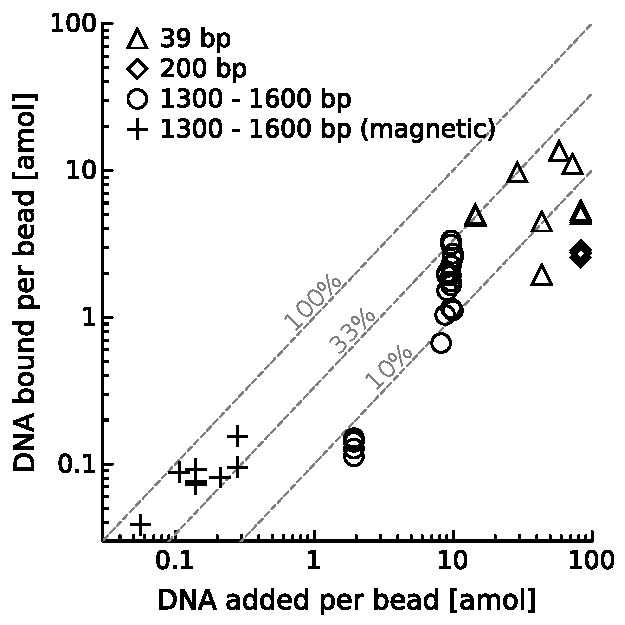
\includegraphics[width=0.4\textwidth]{figures/fig_dna.pdf}
\end{center}
\vspace*{-7mm} % reduce space between labeling and the figure
\caption % This is what goes into Table of Content:
    [\label{sfig:bulkconcat} Expression from bound and unbound DNA fragments.]
    { % This is the text displayed below the figure:
      Comparison of cell-free expression levels from bound and unbound dsDNA.
    } 
\end{figure}

\subsection*{Conclusion}

Your conclusion

%%%%%%%%%%%%%%%%%%%%%%%%%%%%%%%%%%%%%%%%%%%%%%%%%%%%%%%%%%%%%%%%%%%%%
% ACKNOWLEDGEMENTS 
%%%%%%%%%%%%%%%%%%%%%%%%%%%%%%%%%%%%%%%%%%%%%%%%%%%%%%%%%%%%%%%%%%%%%
\section*{Acknowledgements}

This work was supported by ...


\section*{Author Contributions}

A did this. B did that.


\section*{Competing Financial Interests}

The authors declare no competing financial interests.

%%%%%%%%%%%%%%%%%%%%%%%%%%%%%%%%%%%%%%%%%%%%%%%%%%%%%%%%%%%%%%%%%%%%%
%% The appropriate \bibliography command should be placed here.
%%%%%%%%%%%%%%%%%%%%%%%%%%%%%%%%%%%%%%%%%%%%%%%%%%%%%%%%%%%%%%%%%%%%%
\printbibliography

\end{document}
